\documentclass[11pt]{beamer}

% --- Themes and Packages ---
\usetheme{Madrid}
\usecolortheme{default}
\usepackage[utf8]{inputenc}
\usepackage[T1]{fontenc}
\usepackage{graphicx}
\usepackage{booktabs}
\usepackage{hyperref}
\usepackage{tikz}
\usepackage{pgfgantt}
\usetikzlibrary{shapes.geometric, arrows.meta, positioning, fit, backgrounds}

% --- Title Information ---
\title[Community Notes Effectiveness]{Predicting the Effectiveness of Crowd-Sourced Fact-Checking Using Fine-Tuned LLMs}
\subtitle{A Study on Twitter/X Community Notes}
\author[Madan, Pashkov, Salim]{Mridul Madan(01667156) \and Rafael Pashkov (02183763) \and Md Shahidul Salim(02207019)}
\institute[UMass Lowell]{University of Massachusetts Lowell}
\date{Social Computing Project Proposal}

\begin{document}

% --- Slide 1: Title Slide ---
\begin{frame}
    \titlepage
\end{frame}

% --- Slide 2: Project Overview ---
\begin{frame}
    \frametitle{Project Overview}
    \textbf{Core Idea:} 
    \begin{itemize}
        \item Twitter/X's \textbf{Community Notes} allows collaborative fact-checking.
        \item ``Helpful'' notes evaluated by diverse raters are displayed publicly.
        \item \textbf{Goal:} Fine-tune LLMs to predict whether a Note will be rated ``Helpful''.
        \item Analyze linguistic features of effective notes.
        \item Compare fine-tuning approaches with prompting baselines.
    \end{itemize}
\end{frame}

% --- Slide 3: Why This Is Unique \& Strong ---
\begin{frame}
    \frametitle{Why This Is Unique \& Strong?}
    \begin{itemize}
        \item \textbf{Social Computing:} Focuses on crowdsourcing, collective intelligence, and content moderation.
        \item \textbf{Robust Dataset:} Large-scale, public, and directly from Twitter/X.
        \item \textbf{Novelty:} Most existing work studies the ranking algorithm; we focus on computing \textit{content-based} predictions.
        \item \textbf{Methodology:} Directly leverages LLM fine-tuning and inference.
        \item \textbf{Impact:} Real-world applications for misinformation countermeasures.
    \end{itemize}
\end{frame}

% --- Slide 4: Introduction \& Motivation ---
\begin{frame}
    \frametitle{Introduction \& Motivation}
    \begin{itemize}
        \item \textbf{The Problem:} Misinformation scales faster than professional fact-checking.
        \item \textbf{Community Notes:} Crowd-sourced context specifically designed to bridge ideological divides.
        \item \textbf{The Research Gap:} Little work on predicting note effectiveness relying strictly on the text itself.
        \item \textbf{Why it matters:}
        \begin{itemize}
            \item Training future contributors.
            \item Real-time feedback during note drafting.
            \item Prototyping better crowd-sourced moderation systems.
        \end{itemize}
    \end{itemize}
\end{frame}

% --- Slide 5: Proposed Approach ---
\begin{frame}
    \frametitle{Proposed Approach}
    \begin{itemize}
        \item \textbf{Models:} Fine-tune open-source LLMs (Qwen3-4B-Instruct, Gemma-3-4B-IT).
        \item \textbf{Infrastructure:}
        \begin{itemize}
            \item \textbf{Unsloth AI:} Efficient LoRA adaptation.
            \item \textbf{vLLM:} High-throughput serving/inference.
        \end{itemize}
        \item \textbf{Task:} Binary classification (``Currently Rated Helpful'' vs. ``Not Helpful'').
        \item \textbf{Analytical Aim:} Qualitative analysis of linguistic strategies (e.g., source citation, neutral tone, specificity).
    \end{itemize}
\end{frame}

% --- Slide 5b: Project Workflow Diagram ---
\begin{frame}
    \frametitle{Project Workflow}
    \begin{center}
    \resizebox{\textwidth}{!}{
    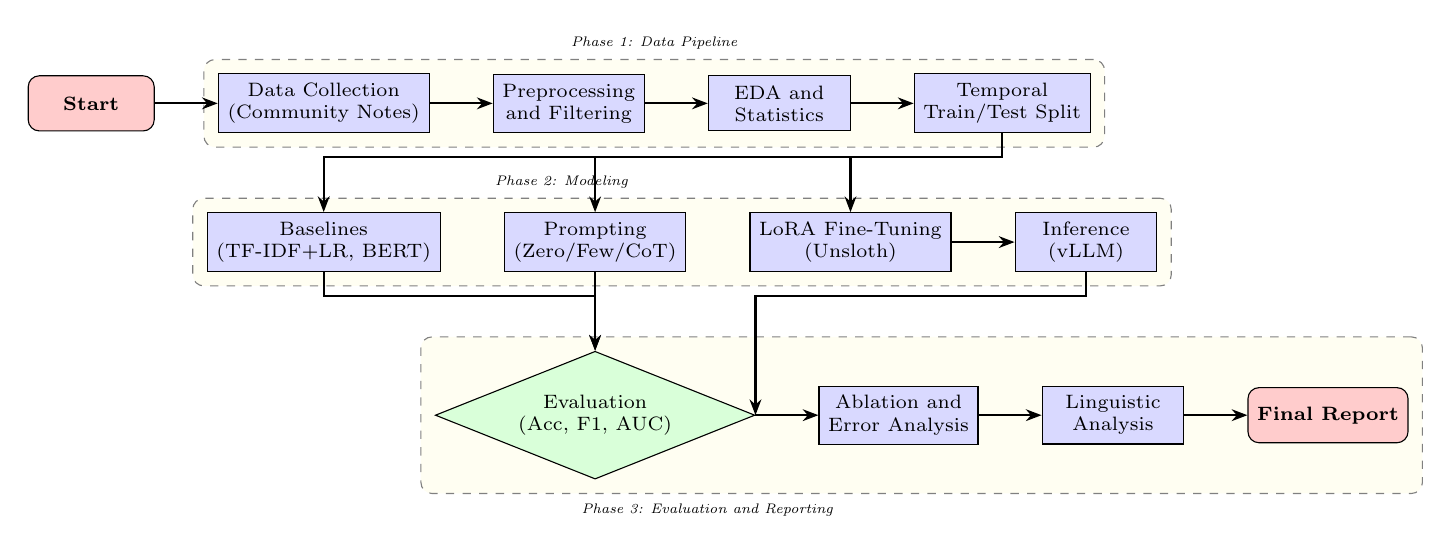
\begin{tikzpicture}[
        node distance=0.4cm and 0.8cm,
        startstop/.style={rectangle, rounded corners, minimum width=1.6cm, minimum height=0.7cm, align=center, draw=black, fill=red!20, font=\scriptsize\bfseries},
        process/.style={rectangle, minimum width=1.8cm, minimum height=0.7cm, align=center, draw=black, fill=blue!15, font=\scriptsize},
        decision/.style={diamond, minimum width=1.4cm, minimum height=0.7cm, align=center, draw=black, fill=green!15, font=\scriptsize, aspect=2.5},
        arrow/.style={-{Stealth[length=2mm]}, thick},
        groupbox/.style={draw=gray, dashed, rounded corners, inner sep=5pt, fill=yellow!5}
    ]
    % Row 1: Data Pipeline
    \node (start) [startstop] {Start};
    \node (collect) [process, right=of start] {Data Collection\\(Community Notes)};
    \node (preprocess) [process, right=of collect] {Preprocessing\\and Filtering};
    \node (eda) [process, right=of preprocess] {EDA and\\Statistics};
    \node (split) [process, right=of eda] {Temporal\\Train/Test Split};

    % Row 2: Model approaches
    \node (baseline) [process, below=1.0cm of collect] {Baselines\\(TF-IDF+LR, BERT)};
    \node (prompting) [process, right=of baseline] {Prompting\\(Zero/Few/CoT)};
    \node (finetune) [process, right=of prompting] {LoRA Fine-Tuning\\(Unsloth)};
    \node (inference) [process, right=of finetune] {Inference\\(vLLM)};

    % Row 3: Evaluation
    \node (eval) [decision, below=1.0cm of prompting] {Evaluation\\(Acc, F1, AUC)};
    \node (ablation) [process, right=of eval] {Ablation and\\Error Analysis};
    \node (linguistic) [process, right=of ablation] {Linguistic\\Analysis};
    \node (report) [startstop, right=of linguistic] {Final Report};

    % Arrows: Row 1
    \draw [arrow] (start) -- (collect);
    \draw [arrow] (collect) -- (preprocess);
    \draw [arrow] (preprocess) -- (eda);
    \draw [arrow] (eda) -- (split);

    % Arrows: Row 1 to Row 2
    \draw [arrow] (split.south) -- ++(0,-0.3) -| (baseline.north);
    \draw [arrow] (split.south) -- ++(0,-0.3) -| (prompting.north);
    \draw [arrow] (split.south) -- ++(0,-0.3) -| (finetune.north);

    % Arrows: Row 2
    \draw [arrow] (finetune) -- (inference);

    % Arrows: Row 2 to Row 3
    \draw [arrow] (baseline.south) -- ++(0,-0.3) -| (eval.north);
    \draw [arrow] (prompting.south) -- (eval.north);
    \draw [arrow] (inference.south) -- ++(0,-0.3) -| (eval.east);

    % Arrows: Row 3
    \draw [arrow] (eval) -- (ablation);
    \draw [arrow] (ablation) -- (linguistic);
    \draw [arrow] (linguistic) -- (report);

    % Group boxes
    \begin{scope}[on background layer]
        \node[groupbox, fit=(collect)(preprocess)(eda)(split), label={[font=\tiny\itshape]above:Phase 1: Data Pipeline}] {};
        \node[groupbox, fit=(baseline)(prompting)(finetune)(inference), label={[font=\tiny\itshape]above left:Phase 2: Modeling}] {};
        \node[groupbox, fit=(eval)(ablation)(linguistic)(report), label={[font=\tiny\itshape]below left:Phase 3: Evaluation and Reporting}] {};
    \end{scope}
    \end{tikzpicture}
    }
    \end{center}
\end{frame}

% --- Slide 6: Dataset ---
\begin{frame}
    \frametitle{Dataset}
    \begin{itemize}
        \item \textbf{Source:} Public Community Notes dataset (updated daily).
        \item \textbf{Key Files \& Variables:}
        \begin{itemize}
            \item \texttt{notes.tsv}: Text (summary), author intent, metadata ($\sim$900K+ notes).
            \item \texttt{ratings.tsv}: Individual helpfulness ratings ($\sim$12M+ ratings).
            \item \texttt{noteStatusHistory.tsv}: Historical labels.
        \end{itemize}
        \item \textbf{Filtering:} Exclude ``NEEDS\_MORE\_RATINGS'' to isolate a concrete binary signal. Estimated ~300K-400K labeled notes.
        \item \textbf{Validation:} \textbf{Temporal split} (e.g., train on past, test on future notes) to simulate real-world deployment and prevent data leakage.
    \end{itemize}
\end{frame}

% --- Slide 6b: Demo Input and Output Example ---
\begin{frame}
    \frametitle{Demo Input and Output Example}
    \textbf{Input (Tweet + Note):}
    \begin{itemize}
        \item[] \textbf{Tweet:} ``The new tax bill will increase taxes for 90\% of Americans next year!''
        \item[] \textbf{Community Note:} ``This claim is misleading. According to the non-partisan Joint Committee on Taxation, taxes will remain unchanged or decrease for 82\% of taxpayers next year. [Link to report]''
    \end{itemize}
    \vspace{0.3cm}
    \textbf{Task Processing (LLM):}
    \begin{itemize}
        \item The model analyzes the note's neutrality, specificity, and presence of authoritative sources against the original tweet context.
    \end{itemize}
    \vspace{0.3cm}
    \textbf{Output (Prediction):}
    \begin{itemize}
        \item[] \textbf{Predicted Status:} \texttt{CURRENTLY\_RATED\_HELPFUL}
        \item[] \textit{Reasoning:} The note cites a credible, non-partisan source, provides specific contrasting figures, and avoids rhetorical attacks.
    \end{itemize}
\end{frame}

% --- Slide 7: Evaluation Framework ---
\begin{frame}
    \frametitle{Evaluation Method}
    \begin{itemize}
        \item \textbf{Quantitative Metrics:}
        \begin{itemize}
            \item \textit{Overall:} Accuracy
            \item \textit{Imbalance constraints:} Precision, Recall, F1-score
            \item \textit{Threshold-independent:} AUC-ROC, AUC-PR
        \end{itemize}
        \vspace{0.5cm}
        \item \textbf{Additional Analyses:}
        \begin{itemize}
            \item \textbf{Ablation Study:} Impact of note length, URL presence, classification task type.
            \item \textbf{Error Analysis:} Investigating common failure modes in the best model.
            \item \textbf{Cross-temporal Generalization.}
        \end{itemize}
    \end{itemize}
\end{frame}

% --- Slide 8: Experimental Comparisons ---
\begin{frame}
    \frametitle{Experimental Comparisons}
    \begin{table}[]
        \centering
        \resizebox{\textwidth}{!}{
        \begin{tabular}{@{}lll@{}}
            \toprule
            \textbf{Approach} & \textbf{Model} & \textbf{Details} \\
            \midrule
            \textbf{Baselines}  & TF-IDF + Logistic Regression & Traditional ML \\
                                & BERT-base fine-tuned & Standard transformer \\
            \midrule
            \textbf{Prompting}  & Qwen3-4B-Instruct (Zero-shot) & No fine-tuning \\
                                & Qwen3-4B-Instruct (Few-shot, 5 ex) & In-context learning \\
                                & Qwen3-4B-Instruct (CoT) & Chain-of-thought \\
            \midrule
            \textbf{Fine-Tuning}& Qwen3-4B-Instruct + LoRA (Unsloth) & \textbf{Primary Method} \\
                                & Gemma-3-4B-IT + LoRA (Unsloth) & Architecture comparison \\
            \bottomrule
        \end{tabular}}
    \end{table}
\end{frame}

% --- Slide 9: Timeline (Gantt Chart) ---
\begin{frame}
    \frametitle{Project Timeline}
    \begin{center}
    \begin{ganttchart}[
        hgrid,
        vgrid,
        x unit=0.85cm,
        y unit chart=0.50cm,
        title height=1,
        bar/.append style={fill=blue!40},
        bar label font=\scriptsize,
        title label font=\scriptsize\bfseries,
        milestone label font=\scriptsize\itshape,
        milestone/.append style={fill=red!60, shape=diamond},
        group/.append style={fill=orange!30},
        group label font=\scriptsize\bfseries
    ]{1}{6}
        \gantttitle{Project Timeline (Weeks)}{6} \\
        \gantttitlelist{1,...,6}{1} \\
        % Phase 1
        \ganttgroup{Phase 1: Data}{1}{1} \\
        \ganttbar{Data Collection \& Preprocessing}{1}{1} \\
        \ganttbar{EDA \& Statistics}{1}{1} \\
        \ganttmilestone{Dataset Ready}{1} \\
        % Phase 2
        \ganttgroup{Phase 2: Modeling}{2}{4} \\
        \ganttbar{Baselines (TF-IDF, BERT)}{2}{2} \\
        \ganttbar{Prompting (Zero/Few-shot, CoT)}{3}{3} \\
        \ganttbar{LoRA Fine-Tuning (Unsloth)}{4}{4} \\
        \ganttmilestone{Models Trained}{4} \\
        % Phase 3
        \ganttgroup{Phase 3: Evaluation}{5}{6} \\
        \ganttbar{Evaluation and Ablation}{5}{5} \\
        \ganttbar{Linguistic Analysis}{5}{6} \\
        \ganttbar{Report Writing}{6}{6} \\
        \ganttmilestone{Final Deliverable}{6}
        % Links
        \ganttlink{elem3}{elem5}
        \ganttlink{elem5}{elem6}
        \ganttlink{elem6}{elem7}
        \ganttlink{elem8}{elem10}
        \ganttlink{elem10}{elem11}
        \ganttlink{elem11}{elem12}
    \end{ganttchart}
    \end{center}
\end{frame}

% --- Slide 10: Division of Labor ---
\begin{frame}
    \frametitle{Division of Labor}
    \begin{itemize}
        \item \textbf{Md Shahidul Salim:}
        \begin{itemize}
            \item LLM fine-tuning (LoRA via Unsloth).
            \item Model training and inference serving (vLLM).
        \end{itemize}
        \vspace{0.3cm}
        \item \textbf{Rafa Pashkov:}
        \begin{itemize}
            \item Data preprocessing and EDA.
            \item Implementation of traditional baselines.
        \end{itemize}
        \vspace{0.3cm}
        \item \textbf{Mridul Madan:}
        \begin{itemize}
            \item Prompting experiments (Zero/Few-shot, CoT).
            \item Evaluation metrics, analysis, and visualizations.
        \end{itemize}
    \end{itemize}
\end{frame}

% --- Slide 11: References ---
\begin{frame}[allowframebreaks]
    \frametitle{References}
    \begin{thebibliography}{5}
        \bibitem{allen2022}
        J. Allen, C. Martel, and D. G. Rand.
        \newblock \emph{Birds of a Feather Don't Fact-Check Each Other: Partisanship and the Evaluation of News in Twitter's Birdwatch Crowdsourced Fact-Checking Program.}
        \newblock CHI 2022.

        \bibitem{chuai2024}
        Y. Chuai, H. Tian, N. Pr\"{o}llochs, and G. Lenzini.
        \newblock \emph{Did the Roll-Out of Community Notes Reduce Engagement With Misinformation on X/Twitter?}
        \newblock CSCW 2024.

        \bibitem{saeed2022}
        M. Saeed, N. Traub, M. Nicolas, G. Demartini, and P. Papotti.
        \newblock \emph{Crowdsourced Fact-Checking at Twitter: How Does the Crowd Compare With Experts?}
        \newblock CIKM 2022.

        \bibitem{vllm}
        B. Hanindhito, B. Patel, and L. K. John.
        \newblock \emph{Large Language Model Fine-tuning with Low-Rank Adaptation: A Performance Exploration.}
        \newblock ICPE 2025.

        \bibitem{unsloth}
        D. Han and M. Han.
        \newblock \emph{Unsloth: Efficient LLM Fine-Tuning.}
        \newblock \url{https://github.com/unslothai/unsloth}, 2024.
    \end{thebibliography}
\end{frame}

% --- Slide 12: Conclusion ---
\begin{frame}
    \frametitle{Conclusion}
    \begin{center}
        \Large \textbf{Thank You!} \\
        \vspace{1cm}
        \normalsize \textbf{Questions?}
    \end{center}
\end{frame}

\end{document}
